\documentclass[11pt]{article}
\usepackage[T1]{fontenc}
\usepackage[utf8]{inputenc}
\usepackage{lmodern,amsmath,graphicx,booktabs,geometry,caption,placeins,xr}
\geometry{margin=2.2cm}
\externaldocument[]{../main/main}
\graphicspath{{../../figures/supplement/}}
\newcommand{\rate}{\ensuremath{\mathrm{m\,a^{-1}}}}
\newcommand{\volrate}{\ensuremath{\mathrm{m^3\,a^{-1}}}}
\renewcommand{\thefigure}{S\arabic{figure}}
\renewcommand{\thetable}{S\arabic{table}}
\renewcommand{\theequation}{S\arabic{equation}}
\begin{document}
\section*{Supplement: additional diagnostic figures}
Supplement to ``A hybrid hypsometric--machine learning approach for reconstructing glacier surface elevation change'' (C. Markovsky, S. Rupper, S. Brewer, and R. R. Forster).

Figure~\ref{fig:relative} shows the sensitivity of relative method improvements to spatial-block width.

\begin{figure}[!htbp]\centering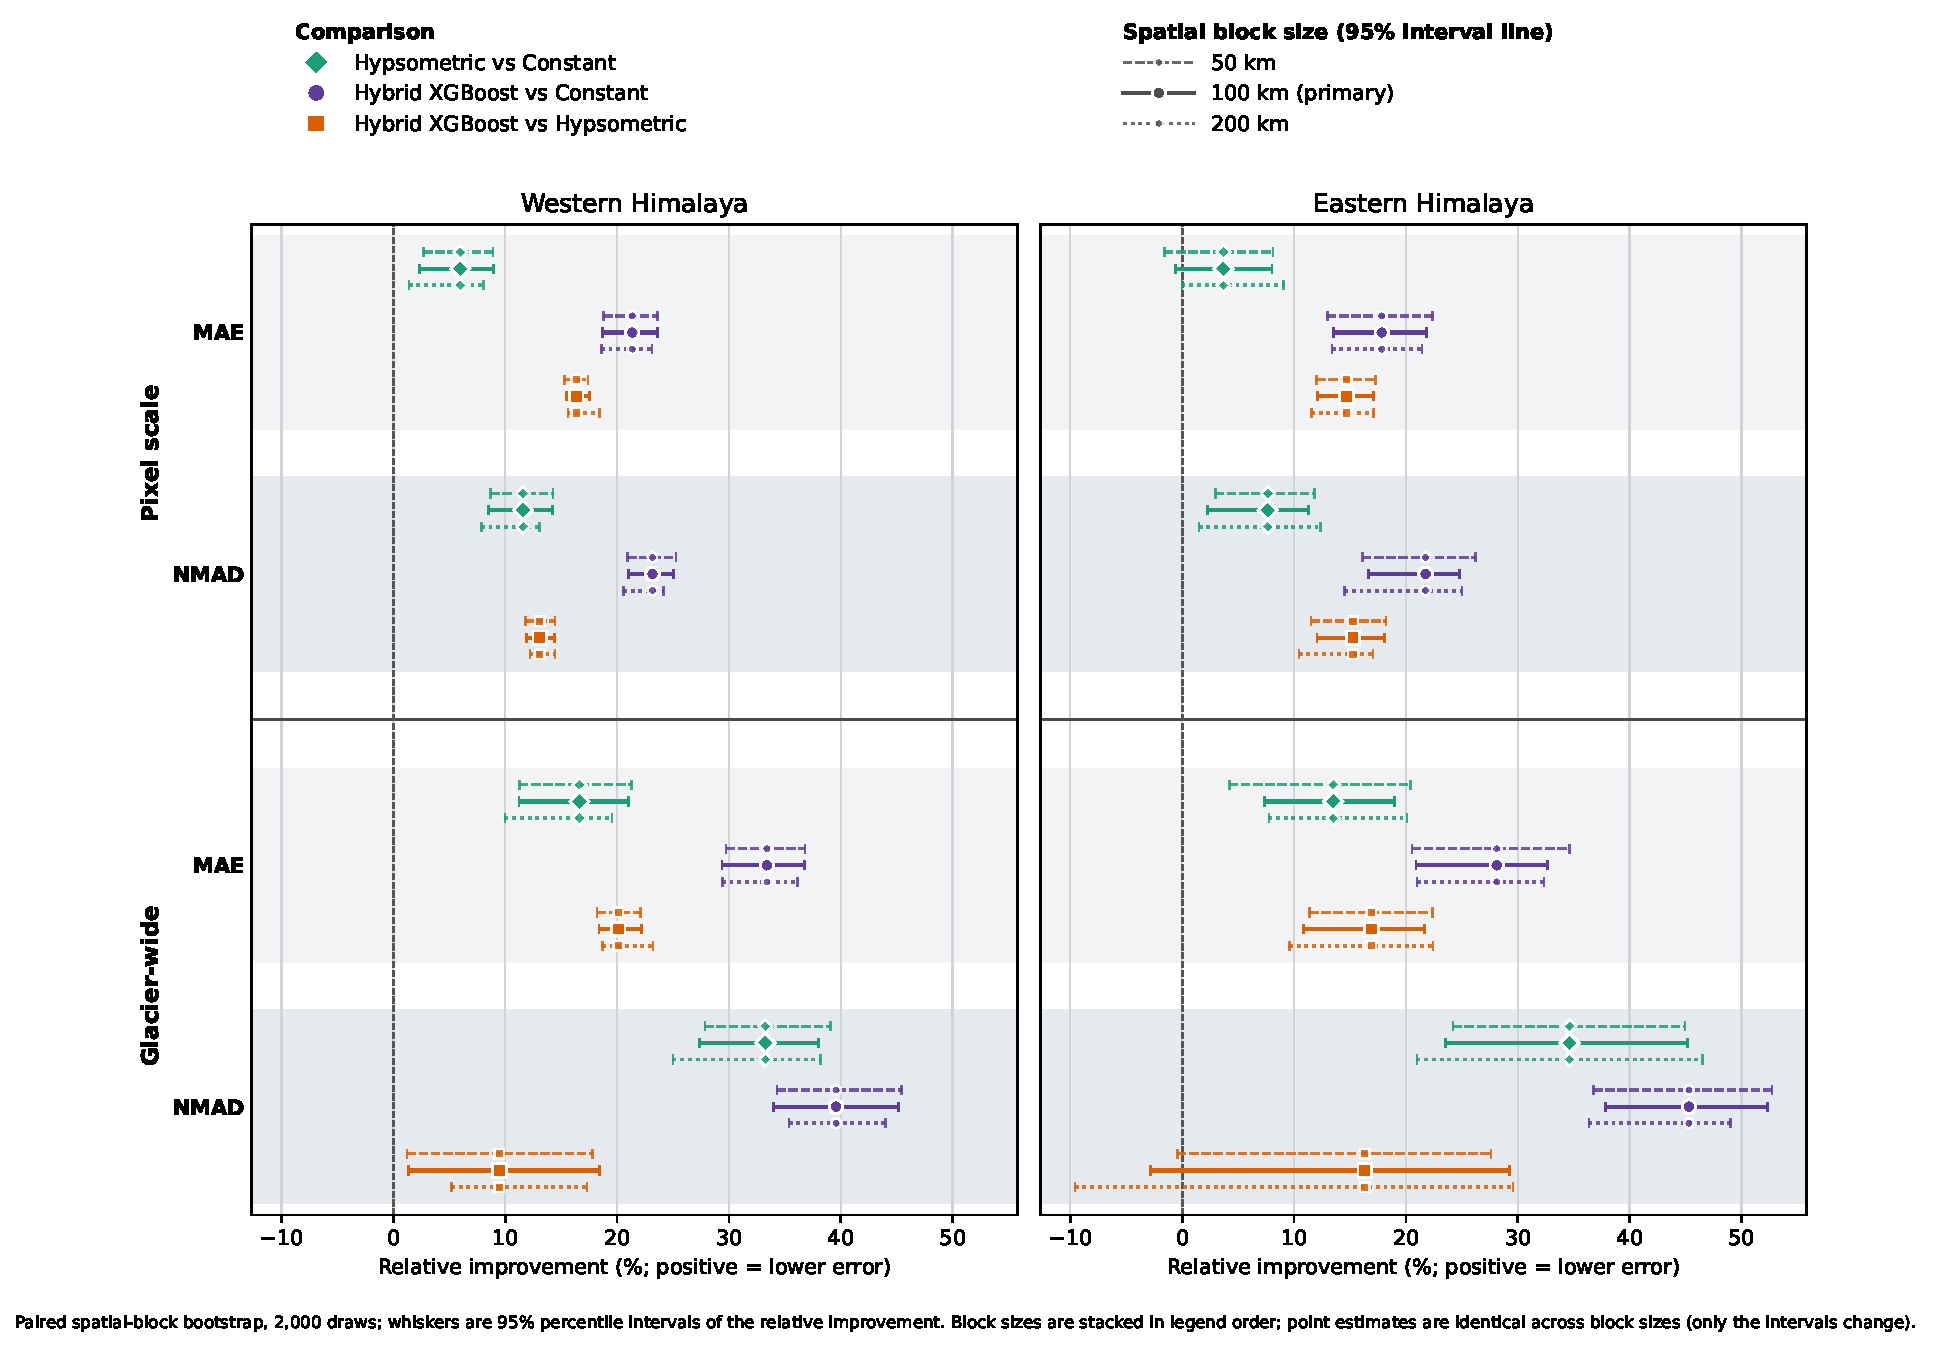
\includegraphics[width=\textwidth,height=.65\textheight,keepaspectratio]{figS01_relative_improvement.pdf}\caption{Relative reductions in pixel and glacier-wide specific MAE and NMAD for the Western (left) and Eastern (right) Himalaya. Colors identify the method pairs in the legend. Reduction is $100(M_{\mathrm{baseline}}-M_{\mathrm{comparison}})/M_{\mathrm{baseline}}$, so positive values favor the comparison method. Bars show 95\% percentile intervals from 2,000 paired spatial-block bootstrap draws at block widths of 50, 100, and 200 km. The point estimate is unchanged across block widths. Each draw uses paired methods and retains all realizations of each glacier. The evaluated test population excludes RGI60-14.17287. Absolute-bias ratios are omitted because near-zero baseline biases make them unstable. Absolute contrasts are shown in Fig.~\ref{fig:bootstrap} and Table~\ref{tab:paired}.}\label{fig:relative}\end{figure}
\clearpage

\begin{figure}[!htbp]\centering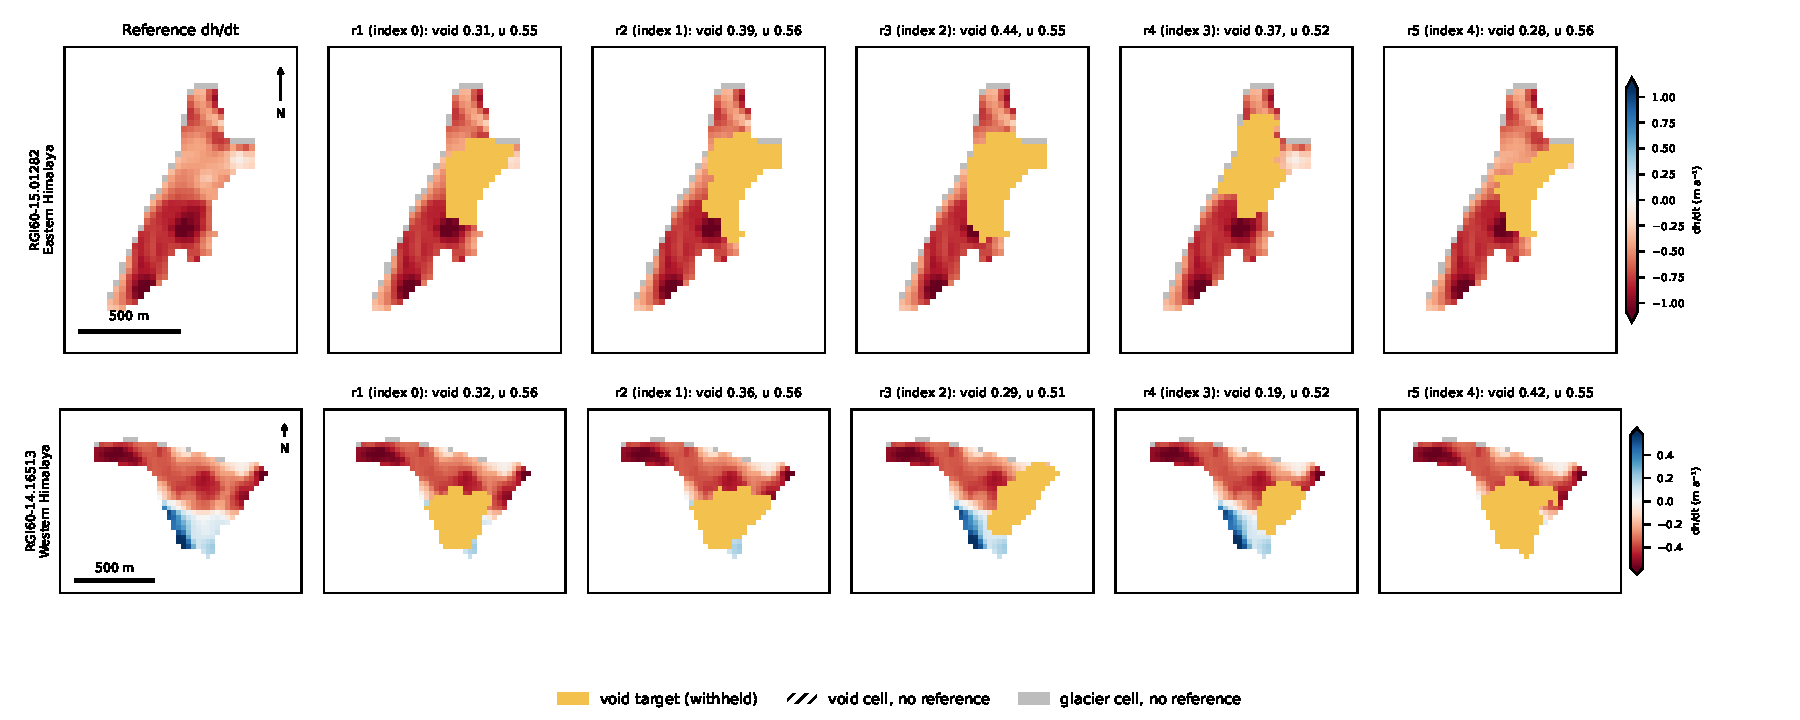
\includegraphics[width=\textwidth,height=.65\textheight,keepaspectratio]{figS02_void_realizations.pdf}\caption{Five retained artificial-void realizations for one geometry-selected glacier per region. Available reference values and native missing support are distinguished; masks may overlap and are processed separately.}\label{fig:masks}\end{figure}
\clearpage

\begin{figure}[!htbp]\centering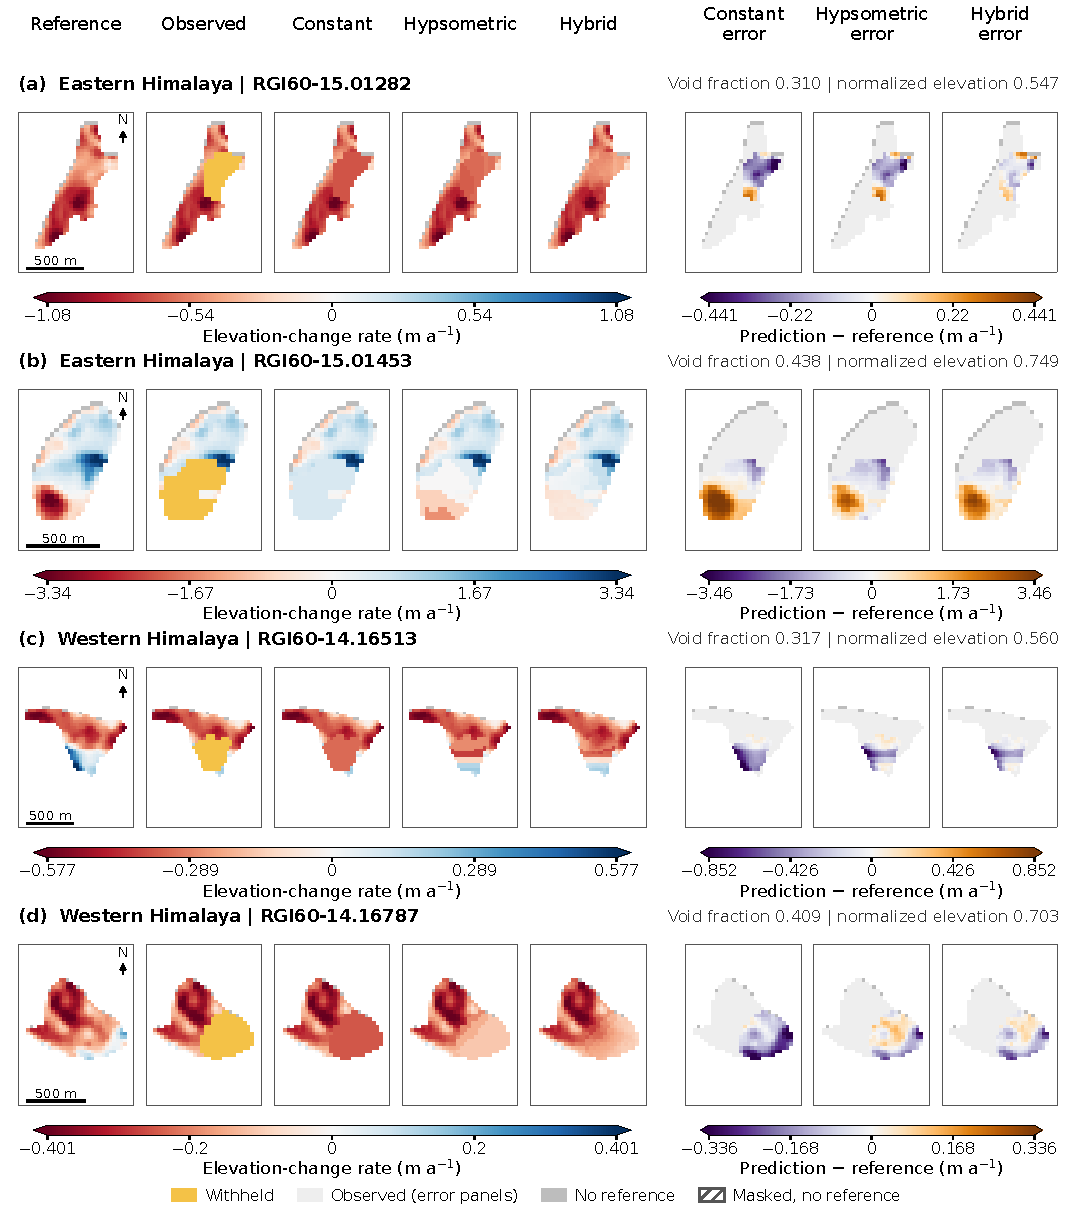
\includegraphics[width=\textwidth]{figS03_reconstruction_examples.pdf}\caption{Reconstruction examples for an artificial-void realization on four test glaciers in the Eastern (a,b) and Western (c,d) Himalaya. Columns show reference elevation-change rates, observations with withheld pixels in yellow, constant, hypsometric, and hybrid reconstructions, and their prediction-minus-reference errors on withheld pixels. Purple and orange errors indicate underestimation and overestimation, respectively. Light gray in error panels marks observed pixels, and dark gray marks pixels without reference data. Each row has separate rate and error colorbars shared across methods. Row headings give achieved void fraction and mean normalized elevation of withheld pixels. Scale bars are 500 m. N indicates projected grid north. These geometry-selected cases illustrate spatial behavior and do not represent the test population.}\label{fig:examples}\end{figure}
\clearpage

\begin{figure}[!htbp]\centering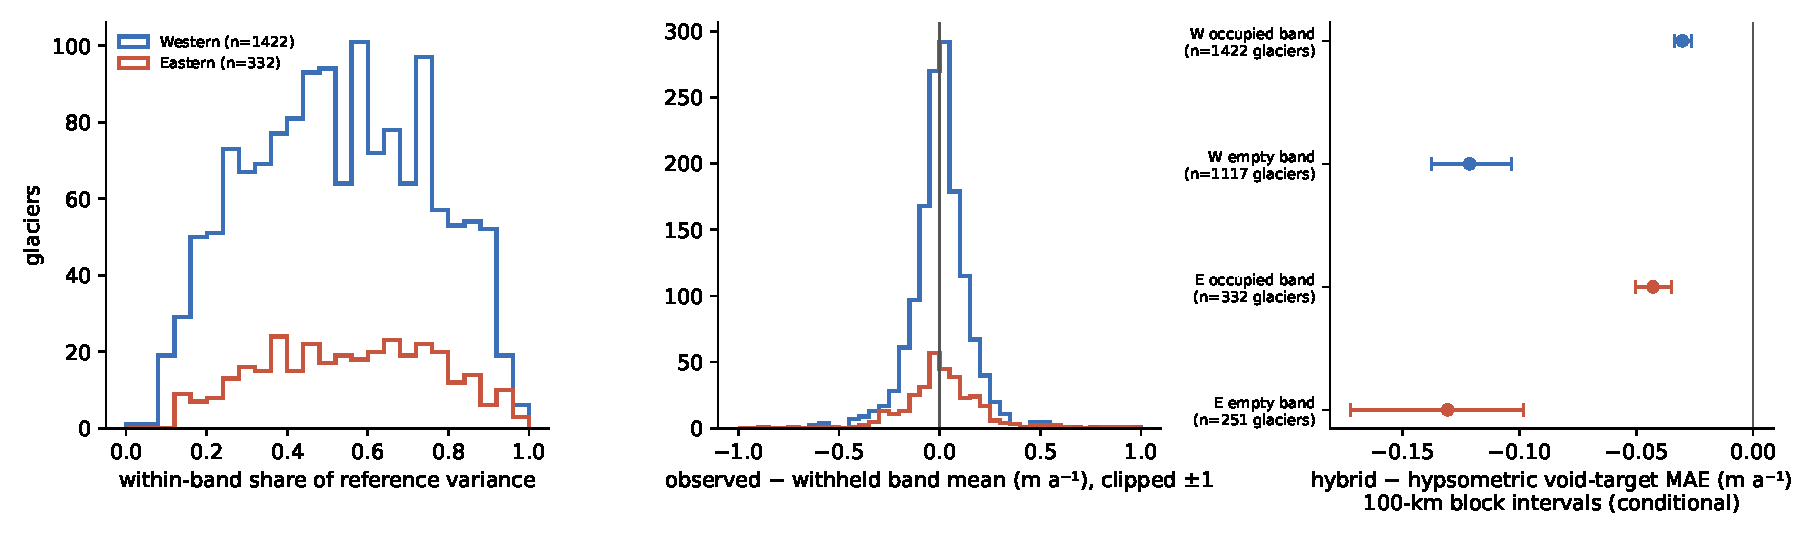
\includegraphics[width=\textwidth,height=.65\textheight,keepaspectratio]{figS04_band_diagnostics.pdf}\caption{Elevation-band variance decomposition, observed/withheld contrasts, and conditional method errors on the evaluated test population of 1,754 glaciers, excluding RGI60-14.17287. Within-band variance is not a measure of predictable physical signal. Restricted-stratum summaries differ from full-support headline metrics.}\label{fig:bands}\end{figure}
\clearpage

\begin{figure}[!htbp]\centering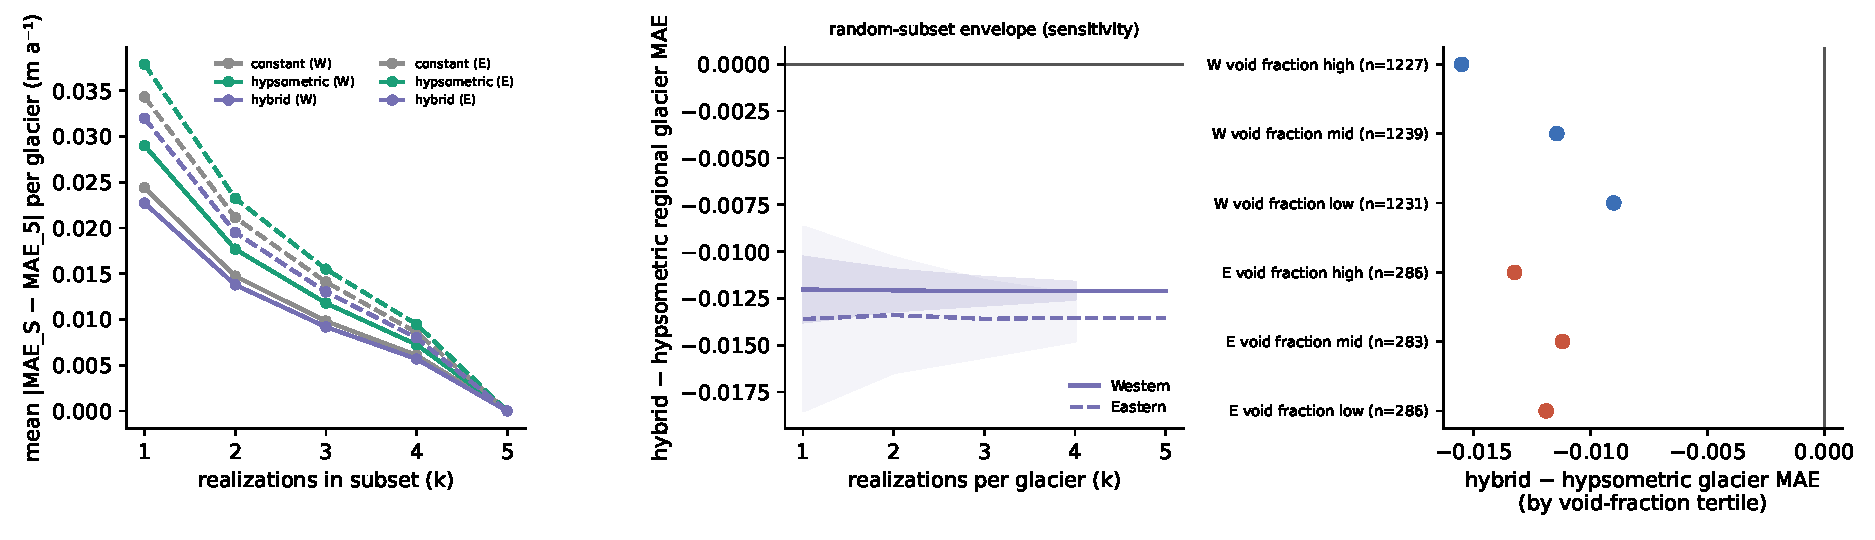
\includegraphics[width=\textwidth,height=.65\textheight,keepaspectratio]{figS05_realization_geometry.pdf}\caption{Sensitivity to subsets of the five retained realizations and achieved void geometry. Regional subset envelopes describe mask sensitivity rather than sampling confidence intervals. All methods use the same subset within each comparison. The evaluated test population excludes RGI60-14.17287, and void-geometry groups keep their original tertile boundaries.}\label{fig:realizations}\end{figure}
\clearpage

\begin{figure}[!htbp]\centering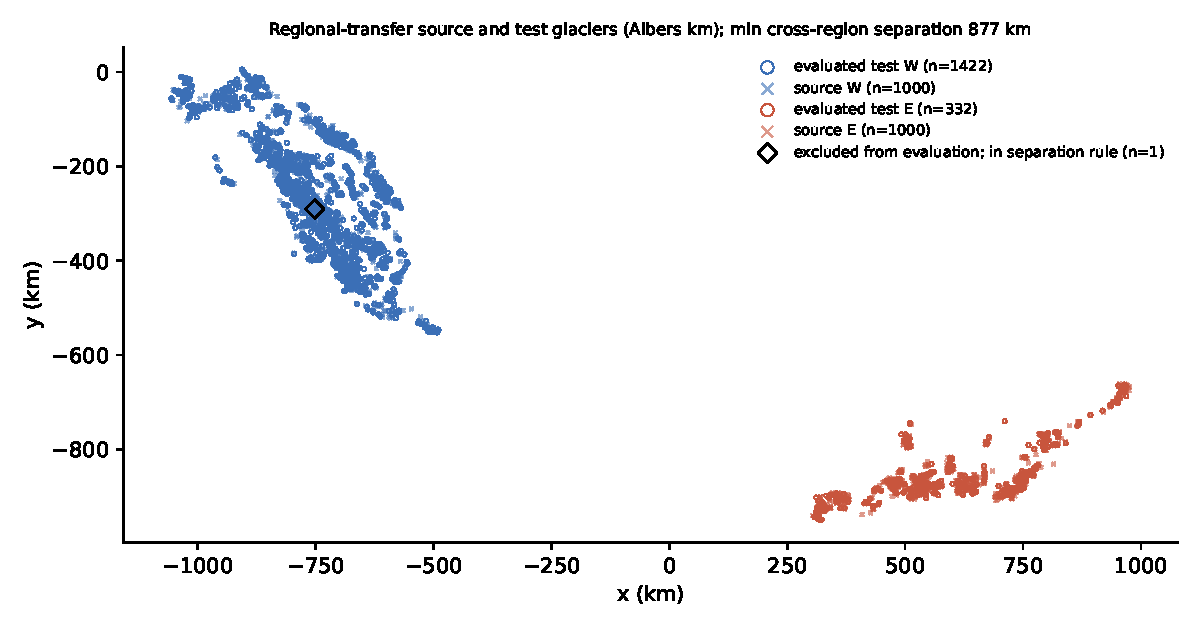
\includegraphics[width=\textwidth,height=.65\textheight,keepaspectratio]{figS06_transfer_separation_map.pdf}\caption{Source samples and target regions for the post hoc regional-transfer sensitivity. The source selection uses metadata and a 100 km exclusion rule from the other region; local target-glacier observations remain available at prediction time. Circles show the 1,754 evaluated test glaciers. The open diamond marks RGI60-14.17287, which is excluded from performance summaries but belonged to the assigned test set used by the locked separation rule.}\label{fig:transfer}\end{figure}
\clearpage

\begin{figure}[!htbp]\centering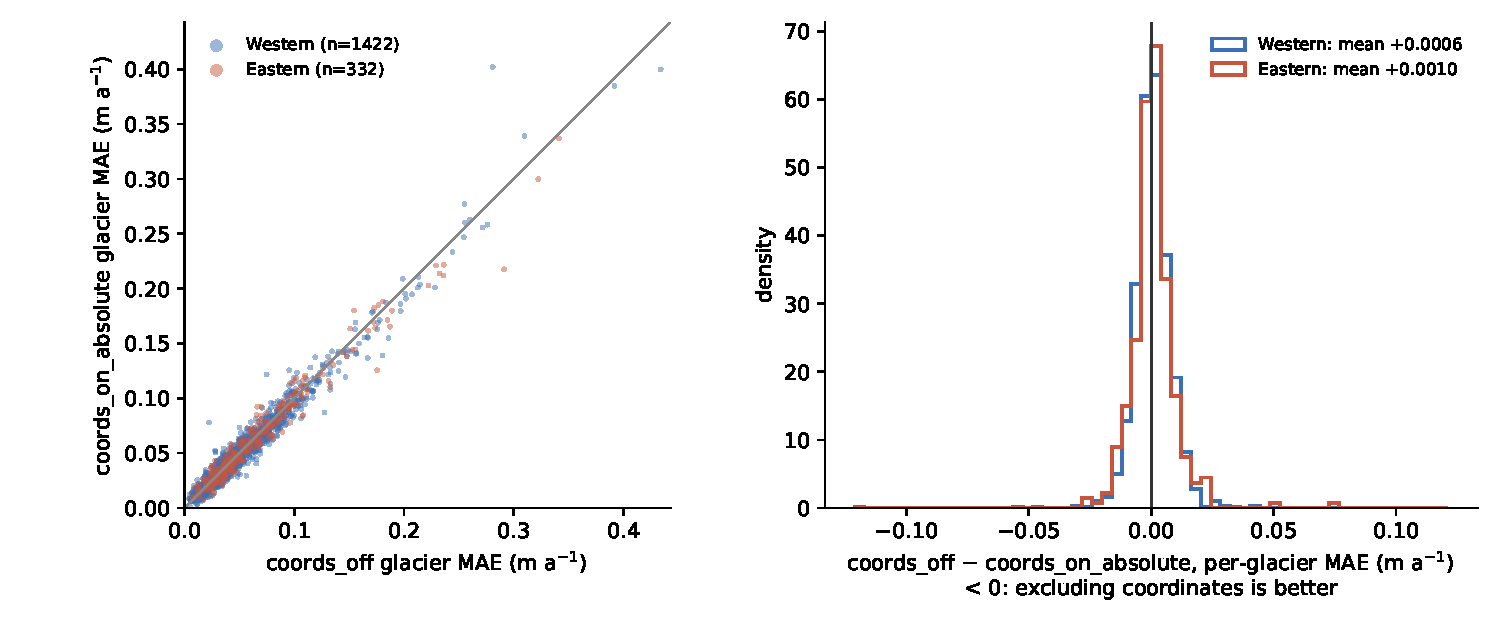
\includegraphics[width=\textwidth,height=.65\textheight,keepaspectratio]{figS07_coordinate_per_glacier.pdf}\caption{Matched coordinate-off and coordinate-on glacier MAE on the evaluated test population of 1,754 glaciers. Both arms use the same capped training sample and fixed settings. Positive off-minus-on differences favor coordinate inclusion. Full data ranges are shown; no display clipping is applied.}\label{fig:coordinates}\end{figure}
\clearpage

\begin{figure}[!htbp]\centering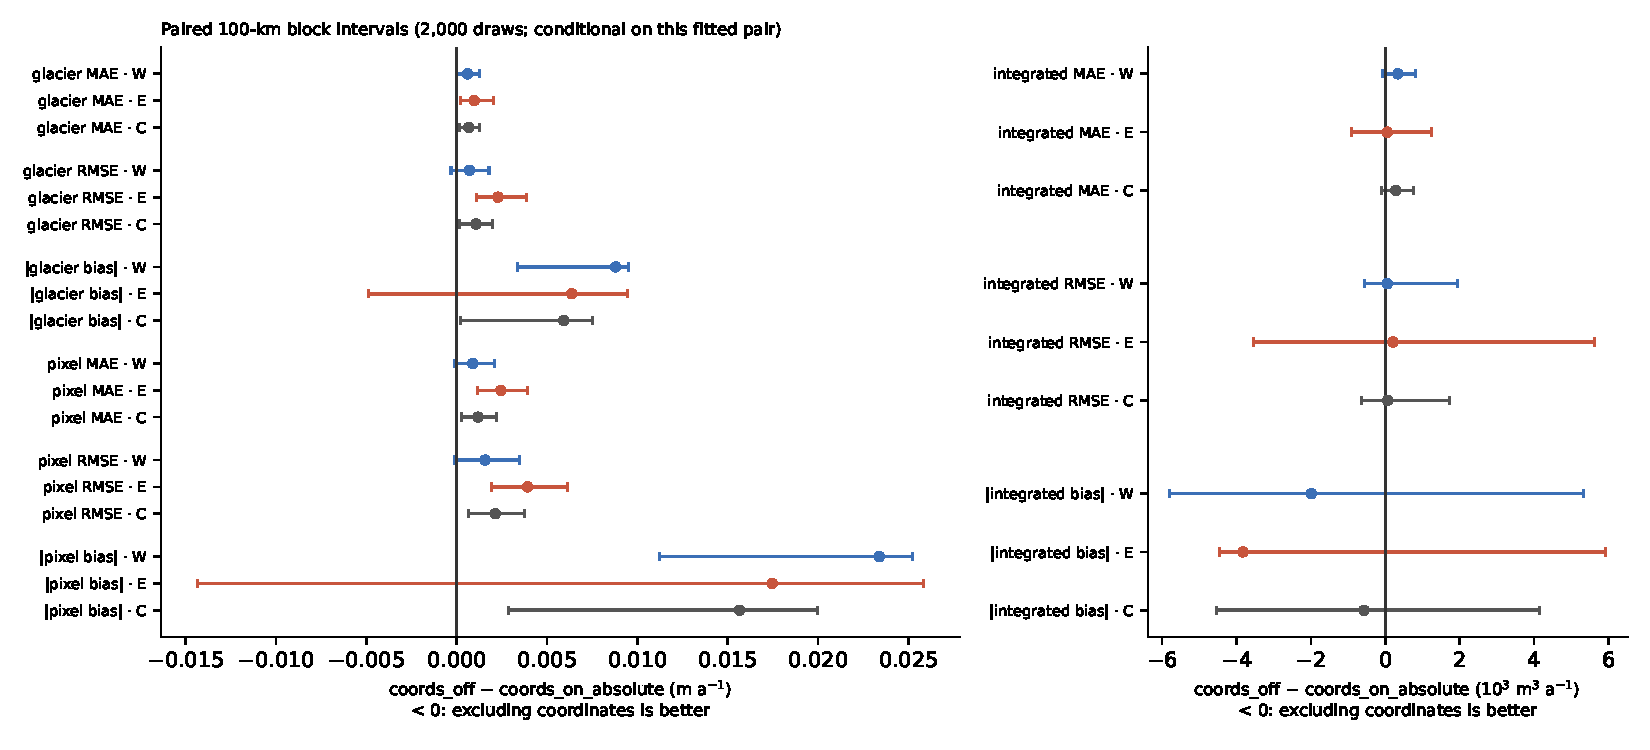
\includegraphics[width=\textwidth,height=.65\textheight,keepaspectratio]{figS08_coordinate_intervals.pdf}\caption{Paired 100 km intervals for the fixed coordinate-model pair. Contrasts are off minus on, with absolute regional bias used for bias-magnitude contrasts. The intervals do not include training variability. Western draws precede Eastern draws from one random-number generator, and the combined interval is region-stratified. The evaluated test population excludes RGI60-14.17287.}\label{fig:coordinateintervals}\end{figure}

\end{document}
